\chapter{Software Architecture}
\label{ch:Software_Architecture}

\author{Nico Kratky}
%

After studying lots of literature about real-time systems, a new fundamental software architecture was developed. The main principle of this is to seperate different tasks into seperate processes. This makes use of the fact that the processed data is sent to the client over the internet anyways. Therefore the process that handles data storage also acts as a client. This leads to increased protability, and more important, increased performance. This sofware stack is depicted in figure \vref{fig:software_architecture}.

\begin{figure}[h]
    \centering
    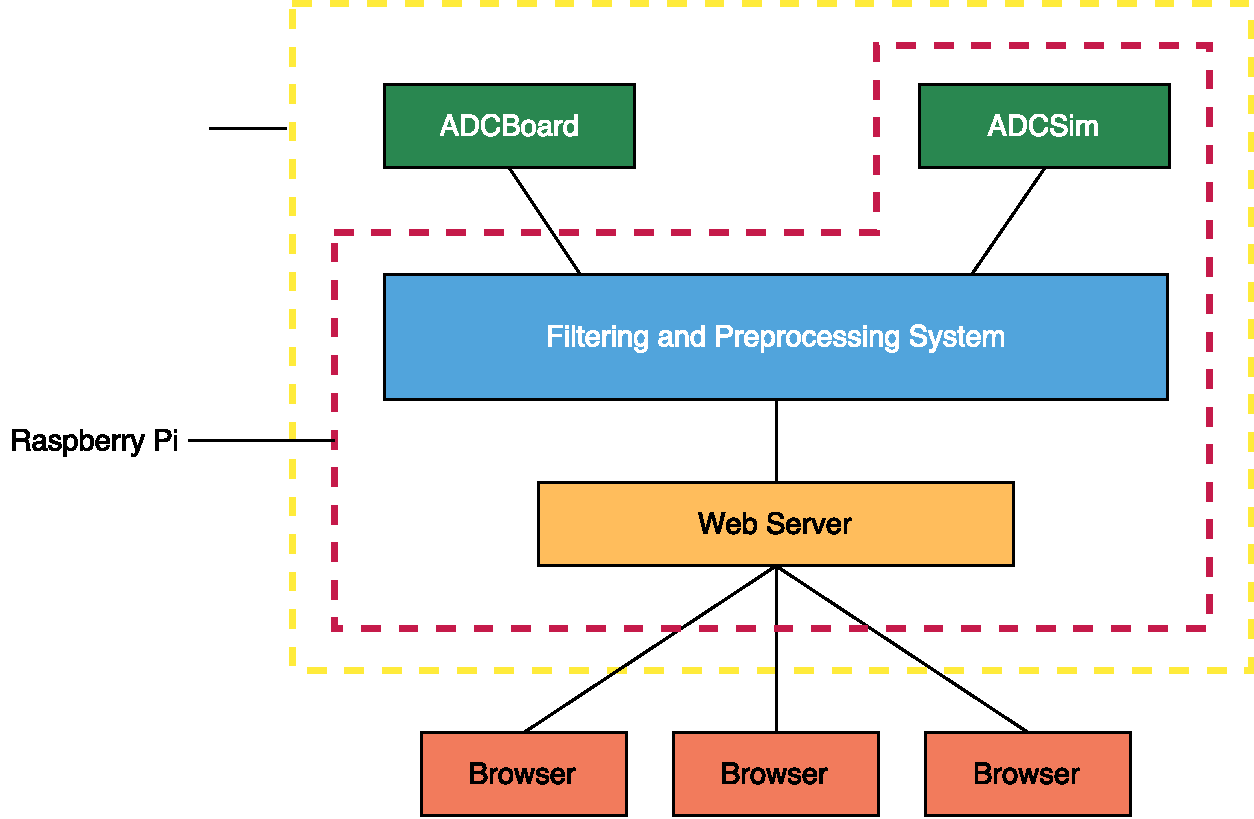
\includegraphics[width=13cm,keepaspectratio]{software_architecture}
    \caption{GRAMOC Software Architecture Diagram}
    \label{fig:software_architecture}
\end{figure}

% \section{Readout}

% Sensor data is read from a gradient magnetometer. This input is already split into six channels and only has to be converted properly. There are two main inputs that can be used with GRAMOC. The real ADC board and ADCSim, which simulates the board.

% \subsection{ADC Board}

% This is the component that handles analog to digital conversion, hence ADC board. This circuit board receives analog data from the sensor in six channels. The first three channels being the magnetic field and the last three the gradientsin xy, xz and yz direction.

% \subsection{Simulator}

% Because the ADC board and a real sensor was not available at all times a simple way of data generation had to be created. Therefore a small application written in C++ was built. This application generates random values and transmits it via UPD just like the real ADC board. Data range and frequency can be adjusted by the user. Another feature that was very important during the development process was the seamless interchangeability with the ADC board.
